\documentclass[12pt,a4paper]{scrartcl}
% Formatvorgaben übernommen aus der früheren Fassung (Drive: Masterarbeit/masterthesis2)
\usepackage[a4paper,top=25mm,bottom=25mm,left=30mm,right=25mm]{geometry}
\usepackage[onehalfspacing]{setspace}
\usepackage{fontspec}
% Deutsch als Hauptsprache; ohne Paket babel-german über die ini-Dateien von babel
\IfFileExists{ngerman.ldf}{\usepackage[english,ngerman]{babel}}{\usepackage[english]{babel}\babelprovide[main,import]{ngerman}}
\usepackage{csquotes}
\usepackage{enumitem}
\usepackage{xcolor,graphicx,float,url}
\usepackage{amsmath,amssymb}
\usepackage{tabularx,booktabs,array,longtable}
\usepackage{tikz}
\usetikzlibrary{arrows.meta,positioning,shapes.geometric}
\usepackage{pgfplots}
\pgfplotsset{compat=1.18}
\usepackage{footnote}
\makesavenoteenv{tabular}
\makesavenoteenv{table}
\usepackage{listings,tcolorbox}
\tcbuselibrary{listingsutf8}
\usepackage[locale=DE]{siunitx}
\usepackage[hidelinks]{hyperref}
\usepackage[labelfont=bf]{caption}
\usepackage[nottoc,notlot,notlof]{tocbibind}
\usepackage[headsepline=true]{scrlayer-scrpage}
\clearpairofpagestyles\ihead{\headmark}\ohead{\pagemark}\cfoot{}\pagestyle{scrheadings}
\setlength{\parskip}{3pt}\parindent 0mm
\setcounter{tocdepth}{3}
\counterwithin{figure}{section}\counterwithin{table}{section}
\newcolumntype{Y}{>{\raggedright\arraybackslash}X}
\newcommand{\simclearpage}{\clearpage\thispagestyle{empty}\vspace*{\fill}\begin{center}\textbf{Diese Seite wurde absichtlich freigelassen.}\end{center}\vspace*{\fill}\clearpage}
% Markierung offener Stellen im Entwurf (vor Abgabe entfernen)
\newcommand{\offen}[1]{\textcolor{red}{\textbf{[OFFEN: #1]}}}


\begin{document}
\thispagestyle{empty}
{\IfFontExistsTF{Times New Roman}{\fontspec{Times New Roman}}{}
\begin{center}
    \IfFileExists{assets/branding/hm_logo.pdf}{\includegraphics[height=1.8cm]{assets/branding/hm_logo.pdf}}{\fbox{HM-Logo fehlt (siehe README)}}\vspace*{0.4cm}\\
    {\normalsize \textbf{MUNICH UNIVERSITY OF APPLIED SCIENCES}}\vspace*{0.15cm}\\
    {\small FACULTY OF COMPUTER SCIENCE AND MATHEMATICS}
\end{center}
\vspace*{1.8cm}
\begin{center}
    {\normalsize MASTER'S THESIS}\\
    \vspace*{0.15cm}\rule{1.8cm}{1pt}\vspace*{0.4cm}\\
    {\Large \textbf{Regulatorische Anforderungen in KI-gestützten Geschäftsprozessen}\\[0.2cm]
    \textbf{erkennen und zur Laufzeit durchsetzen}}\\[0.6cm]
    {\normalsize Ein LLM-Agent zur Zuordnung von Vorschriften, zur Erkennung von Compliance-Lücken und zur Runtime Verification am Beispiel eines Bewerbungsverfahrens an einer bayerischen Hochschule}
\end{center}
\vspace*{1.3cm}
\begin{center}
    {\Large \textbf{Sebastian Haug}}\\
    {\footnotesize Master's programme}
\end{center}
\vspace*{0.8cm}
\begin{center}
    {\large \textbf{Prof. Dr. Christoph Böhm}}\\
    {\footnotesize Supervisor from Munich University of Applied Sciences}
\end{center}
\vfill
\begin{center}{\footnotesize Munich, \offen{Abgabemonat}}\end{center}
}

\simclearpage
% Platzhalter: In der früheren Fassung identisch mit titlepage.tex. Durch das offizielle HM-Deckblatt ersetzen, falls vorgeschrieben.
\thispagestyle{empty}
{\IfFontExistsTF{Times New Roman}{\fontspec{Times New Roman}}{}
\begin{center}
    \IfFileExists{assets/branding/hm_logo.pdf}{\includegraphics[height=1.8cm]{assets/branding/hm_logo.pdf}}{\fbox{HM-Logo fehlt (siehe README)}}\vspace*{0.4cm}\\
    {\normalsize \textbf{MUNICH UNIVERSITY OF APPLIED SCIENCES}}\vspace*{0.15cm}\\
    {\small FACULTY OF COMPUTER SCIENCE AND MATHEMATICS}
\end{center}
\vspace*{1.8cm}
\begin{center}
    {\normalsize MASTER'S THESIS}\\
    \vspace*{0.15cm}\rule{1.8cm}{1pt}\vspace*{0.4cm}\\
    {\Large \textbf{Regulatorische Anforderungen in KI-gestützten Geschäftsprozessen}\\[0.2cm]
    \textbf{erkennen und zur Laufzeit durchsetzen}}\\[0.6cm]
    {\normalsize Ein LLM-Agent zur Zuordnung von Vorschriften, zur Erkennung von Compliance-Lücken und zur Runtime Verification am Beispiel eines Bewerbungsverfahrens an einer bayerischen Hochschule}
\end{center}
\vspace*{1.3cm}
\begin{center}
    {\Large \textbf{Sebastian Haug}}\\
    {\footnotesize Master's programme}
\end{center}
\vspace*{0.8cm}
\begin{center}
    {\large \textbf{Prof. Dr. Christoph Böhm}}\\
    {\footnotesize Supervisor from Munich University of Applied Sciences}
\end{center}
\vfill
\begin{center}{\footnotesize Munich, \offen{Abgabemonat}}\end{center}
}

\simclearpage
\pagenumbering{Roman}\setcounter{page}{1}
\section*{Kurzfassung}\addcontentsline{toc}{section}{Kurzfassung}
\offen{Kurzfassung wird zuletzt geschrieben (Deutsch und Englisch, je ca.\ 200 Wörter).}
\simclearpage
\tableofcontents
\listoffigures\listoftables
\clearpage\printglossar
\clearpage\pagenumbering{arabic}\setcounter{page}{1}

\section{Einleitung}
\subsection{Motivation}
\offen{1.1 Motivation -- Stichpunkte im Entwurf}

\subsection{Problemstellung}
\offen{1.2 Problemstellung -- Stichpunkte im Entwurf}

\subsection{Forschungsfragen und Hypothesen}
% abgesegnet am 27.10.2026
\textbf{Zentrale Forschungsfrage:} Kann ein LLM-Agent für einen Geschäftsprozess die geltenden Vorschriften selbst recherchieren, den Arbeitsschritten zuordnen und fehlende Schritte erkennen -- und lassen sich diese Vorschriften in Prüfregeln übersetzen, die das Verhalten eines KI-Agenten zur Laufzeit kontrollieren?

Die zentrale Forschungsfrage wird entlang einer Kette von fünf Schritten untersucht (Abbildung~\ref{fig:untersuchungskette}). Jeder Schritt verarbeitet das Ergebnis des vorherigen und wird durch eine eigene Hypothese geprüft. Ob die Kette als Ganzes trägt, prüft Hypothese H4.

\begin{figure}[H]
  \centering
  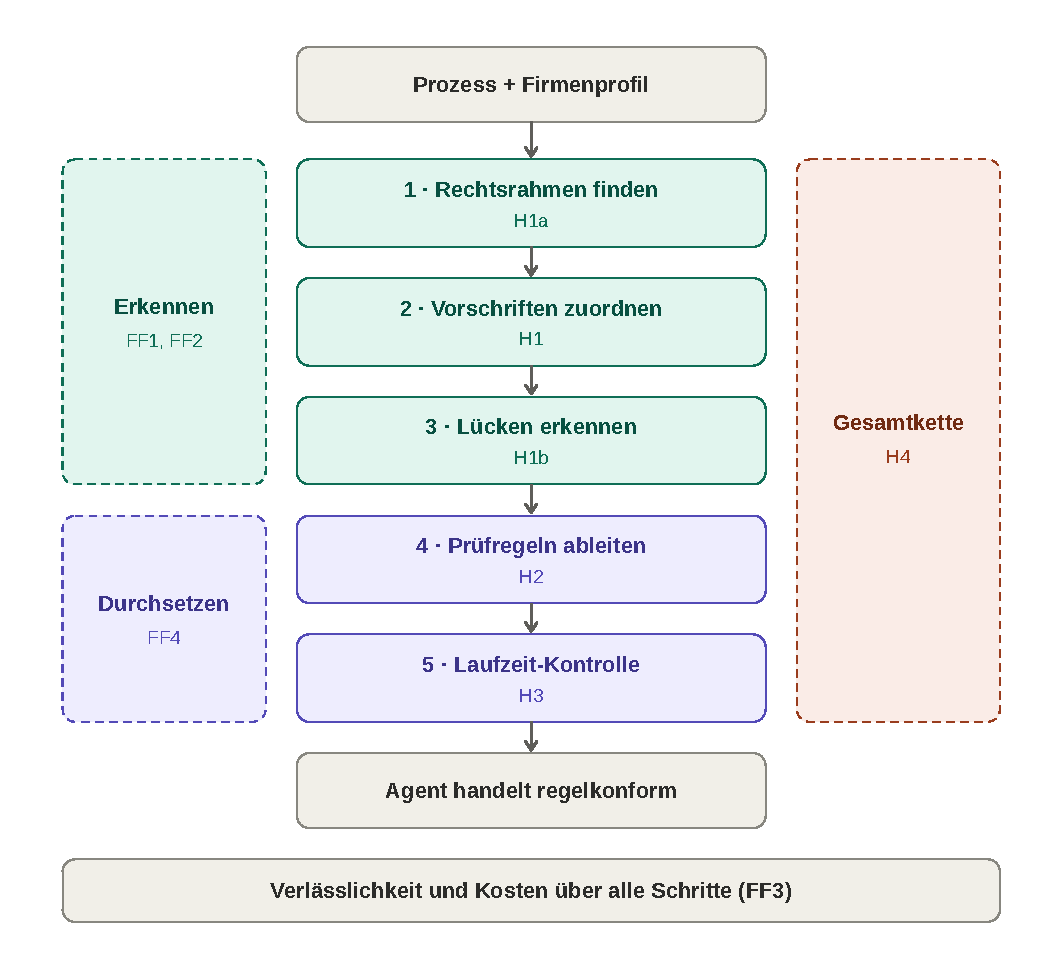
\includegraphics[width=0.85\textwidth]{figures/abb_1_1_untersuchungskette.pdf}
  \caption[Untersuchungskette der Arbeit]{Untersuchungskette der Arbeit. Die Schritte 1 bis 3 erkennen regulatorische Anforderungen, die Schritte 4 und 5 setzen sie zur Laufzeit durch.}
  \label{fig:untersuchungskette}
\end{figure}

\begin{description}[leftmargin=1.2cm,style=nextline]
  \item[FF1] Wie vollständig und wie genau bestimmt ein LLM-Agent mit eigener Recherche die für einen Geschäftsprozess geltenden Regelwerke und ordnet deren Vorschriften den einzelnen Arbeitsschritten zu?
  \begin{description}[leftmargin=1.2cm]
    \item[H1a] Der Agent bestimmt die geltenden Regelwerke nahezu vollständig (\fb{trefferquote} $\geq 0{,}9$).
    \item[H1] Der Agent ordnet die geltenden Vorschriften den Arbeitsschritten mindestens so vollständig zu wie GPT-4 bei Sai et al.~\cite{sai2024} auf Task-Ebene (\fb{trefferquote} $\geq 0{,}62$).
  \end{description}
  \item[FF2] Erkennt der Agent rechtlich gebotene Schritte, die im Prozess fehlen?
  \begin{description}[leftmargin=1.2cm]
    \item[H1b] Der Agent erkennt die Mehrheit der fehlenden Schritte, ohne vorhandene Schritte als fehlend zu melden.
  \end{description}
  \item[FF3] Wie beeinflussen die Gestaltung des Prompts und das Recherchewerkzeug die Vollständigkeit, die Genauigkeit, den Anteil erfundener Normen und die Kosten?
  \item[FF4] Lassen sich die zugeordneten Vorschriften in maschinell prüfbare Regeln übersetzen, mit denen sich das Verhalten eines KI-Agenten zur Laufzeit kontrollieren lässt?
  \begin{description}[leftmargin=1.2cm]
    \item[H2] Aus den zugeordneten Vorschriften lassen sich Prüfregeln erzeugen, die bei Referenzfällen dieselbe Entscheidung treffen wie eine fachliche Prüfung.
    \item[H3] Ein Laufzeitmonitor mit diesen Prüfregeln verhindert unzulässige Aktionen eines KI-Agenten, ohne zulässige Aktionen zu blockieren.
    \item[H4] Auch wenn die Ergebnisse des Agenten aus H1 und H1b unkorrigiert weitergegeben werden, verhindert die Laufzeit-Kontrolle die Mehrheit der unzulässigen Aktionen.
  \end{description}
\end{description}

\subsection{Beitrag der Arbeit}
\offen{1.4 Beitrag}

\subsection{Aufbau der Arbeit}
\offen{1.5 Aufbau -- wird zuletzt geschrieben}

\section{Grundlagen}
\subsection{Geschäftsprozesse}
% Plan 2.1 (Stand 28.10.2026), wird Satz für Satz abgesegnet:
%  1. Was ist ein Geschäftsprozess (Definition mit Quelle)
%  2. Prozesse werden hierarchisch zerlegt: Prozess -> Teilprozess -> Task
%  3. Formale Grundlage BPMN 2.0: Task = atomare Aktivität, Teilprozess = zusammengesetzte Aktivität
%  4. Zahl der Ebenen ist Konvention: APQC PCF nutzt fünf Ebenen
%  5. Warum die Ebenen für Compliance wichtig sind: Vorschriften gelten unterschiedlich weit (ganzer Prozess / Abschnitt / einzelner Schritt)
%  6. Diese Arbeit: drei Ebenen wie Sai et al.; Prozess als strukturierte Liste (1 Prozess, 6 Teilprozesse, 19 Tasks), nicht als BPMN-Grafik
\offen{2.1 -- wird Satz für Satz geschrieben}

\subsection{Regulatorische Compliance}
\offen{2.2}

\subsection{Rechtsrahmen des Anwendungsfalls}
\offen{2.3}

\subsection{Sprachmodelle und Agenten}
\offen{2.4}

\subsection{Bewertungsmaße}
\offen{2.5}

\section{Verwandte Arbeiten}
\subsection{Zuordnung von Vorschriften zu Geschäftsprozessen}
% abgesegnet am 27.10.2026; "am nächsten" nach der Literaturrecherche zu 3.2 prüfen
Am nächsten an dieser Arbeit liegt die Studie von Sai et al.~\cite{sai2024}, die untersucht, wie sich aus einer Sammlung von Rechtstexten automatisch die Absätze bestimmen lassen, die für einen gegebenen Geschäftsprozess relevant sind.

\offen{weitere Sätze zu 3.1}

\subsection{Rechtsinformationssuche mit Sprachmodellen}
\offen{3.2 -- Literaturrecherche}

\subsection{Runtime Verification von Agenten}
\offen{3.3 -- C-Trace}

\subsection{Forschungslücke}
\offen{3.4}

\section{Methodik}
\offen{Kapitel 4 -- Stichpunkte im Entwurf}

\section{Implementierung}
\offen{Kapitel 5 -- Stichpunkte im Entwurf}

\section{Ergebnisse}
\offen{Kapitel 6 -- nach Auftrag 004 (v4)}

\section{Diskussion}
\offen{Kapitel 7 -- Stichpunkte im Entwurf}

\section{Fazit und Ausblick}
\offen{Kapitel 8 -- Stichpunkte im Entwurf}


\clearpage
\bibliographystyle{unsrt}
\bibliography{literatur}
\end{document}
